%%========================================================================
%% LaTeX scriptiesjabloon
%%========================================================================
%%========================================================================
%% Preamble
%%========================================================================

\documentclass[pdftex,a4paper,12pt,twoside]{report}

\usepackage{color}					 % kleur voor syntax highlighting
\usepackage{caption}
\usepackage{subcaption}
\usepackage[utf8]{inputenc}  % Accenten gebruiken in tekst (vb. � ipv \'e)
\usepackage{amsfonts}        % AMS math packages: extra wiskundige
\usepackage{amsmath}         %   symbolen (o.a. getallen-
\usepackage{amssymb}         %   verzamelingen N, R, Z, Q, etc.)
\usepackage[UKenglish]{babel}    % Taalinstellingen: woordsplitsingen,
                             %  commando's voor speciale karakters
                             %  ("dutch" voor NL)
                                                         %  ("UKenglish" voor brits engels)
\usepackage{eurosym}         % Euro-symbool �
\usepackage{graphicx}        % Invoegen van tekeningen
\usepackage[pdftex,bookmarks=true]{hyperref}
                             % PDF krijgt klikbare links & verwijzingen,
                             %  inhoudstafel
\usepackage{listings}        % Broncode mooi opmaken
\usepackage{multirow}        % Tekst over verschillende cellen in tabellen
\usepackage{rotating}        % Tabellen en figuren roteren
\usepackage{natbib}          % Betere bibliografiestijlen
\usepackage{fancyhdr}        % Pagina-opmaak met hoofd- en voettekst
\usepackage{footnote}
\usepackage{parskip}
\usepackage{longtable}			 % For tables longer than one page
\usepackage[final]{pdfpages}

% paragrafen zonder indentatie, en op andere lijn
\setlength{\parindent}{0pt }
\setlength{\parskip}{12pt plus 1pt minus 1pt}


\definecolor{dkgreen}{rgb}{0,0.6,0}
\definecolor{gray}{rgb}{0.5,0.5,0.5}
\definecolor{mauve}{rgb}{0.58,0,0.82}
\definecolor{darkgray}{rgb}{0.662745,0.662745,0.662745}
\definecolor{black}{rgb}{0,0,0}
\definecolor{lightgray}{rgb}{.9,.9,.9}
\definecolor{darkgray}{rgb}{.4,.4,.4}
\definecolor{purple}{rgb}{0.65, 0.12, 0.82}
\definecolor{darkblue}{rgb}{0.0,0.0,0.6}
\definecolor{cyan}{rgb}{0.0,0.6,0.6}


%%---------- Layout ------------------------------------------------------
\newcommand{\includecode}[2][c]{\lstinputlisting[caption=#2, escapechar=]{#2}}

% hoofdingen, enz.
\pagestyle{fancy}

% lijn, wordt gebruikt in titelpagina
\newcommand{\HRule}{\rule{\linewidth}{0.5mm}}

% Leeg blad
\newcommand{\emptypage}
{
	\newpage
	\thispagestyle{empty}
	\mbox{}
	\newpage
}
 
% Gebruik een schreefloos lettertype ipv het "oubollig" uitziende
% Computer Modern
\renewcommand{\familydefault}{\sfdefault}     

% Commando voor invoegen Java-broncodebestanden (dank aan Niels Corneille)
% Gebruik: \codefragment{source/MijnKlasse.java}{Uitleg bij de code}
\newcommand{\codefragmentjava}[2]
{ \lstset{%
  language=java,
  breaklines=true,
  float=th,
  caption={#2},
  basicstyle=\scriptsize,
  frame=single
}
\lstinputlisting{#1}}


\lstset{frame=tb,
  language=Java,
  aboveskip=3mm,
  belowskip=3mm,
  showstringspaces=false,
  columns=flexible,
  basicstyle={\small\ttfamily},
  numbers=left,
  numberstyle=\footnotesize,
  keywordstyle=\color{blue},
  commentstyle=\color{dkgreen},
  stringstyle=\color{mauve},
  breaklines=true,
  breakatwhitespace=true
  tabsize=3,
	captionpos=b,
	extendedchars=true
}

\lstdefinelanguage{JavaScript}
{
  keywords={typeof, new, true, false, catch, function, return, null, catch, switch, var, if, in, while, do, else, case, break},
  keywordstyle=\color{blue}\bfseries,
  ndkeywords={class, export, boolean, throw, implements, import, this},
  ndkeywordstyle=\color{darkgray}\bfseries,
  identifierstyle=\color{black},
  sensitive=false,
  comment=[l]{//},
  morecomment=[s]{/*}{*/},
  commentstyle=\color{purple}\ttfamily,
  stringstyle=\color{red}\ttfamily,
  morestring=[b]',
  morestring=[b]"
}

\lstdefinelanguage{XML}
{
  basicstyle=\ttfamily\color{darkblue}\bfseries,
  morestring=[b]",
  morestring=[s]{>}{<},
  morecomment=[s]{<?}{?>},
  stringstyle=\color{black},
  identifierstyle=\color{darkblue},
  keywordstyle=\color{cyan},
  morekeywords={xmlns,version,type}% list your attributes here
}


\lstdefinelanguage{CSS}
{
	alsodigit={-},
	ndkeywords={@import, @media, @page, @font-face, @charset, @namespace, @viewport, @-ms-viewport, @-o-viewport, @-moz-viewport, @-webkit-viewport, th},
  ndkeywordstyle=\color{darkgray}\bfseries,
  morekeywords={accelerator,azimuth,background,background-attachment,
    background-color,background-image,background-position,
    background-position-x,background-position-y,background-repeat,
    behavior,border,border-bottom,border-bottom-color,
    border-bottom-style,border-bottom-width,border-collapse,
    border-color,border-left,border-left-color,border-left-style,
    border-left-width,border-right,border-right-color,
    border-right-style,border-right-width,border-spacing,
    border-style,border-top,border-top-color,border-top-style,
    border-top-width,border-width,bottom,caption-side,clear,
    clip,color,content,counter-increment,counter-reset,cue,
    cue-after,cue-before,cursor,direction,display,elevation,
    empty-cells,filter,float,font,font-family,font-size,
    font-size-adjust,font-stretch,font-style,font-variant,
    font-weight,height,ime-mode,include-source,
    layer-background-color,layer-background-image,layout-flow,
    layout-grid,layout-grid-char,layout-grid-char-spacing,
    layout-grid-line,layout-grid-mode,layout-grid-type,left,
    letter-spacing,line-break,line-height,list-style,
    list-style-image,list-style-position,list-style-type,margin,
    margin-bottom,margin-left,margin-right,margin-top,
    marker-offset,marks,max-height,max-width,min-height,
    min-width,-moz-binding,-moz-border-radius,
    -moz-border-radius-topleft,-moz-border-radius-topright,
    -moz-border-radius-bottomright,-moz-border-radius-bottomleft,
    -moz-border-top-colors,-moz-border-right-colors,
    -moz-border-bottom-colors,-moz-border-left-colors,-moz-opacity,
    -moz-outline,-moz-outline-color,-moz-outline-style,
    -moz-outline-width,-moz-user-focus,-moz-user-input,
    -moz-user-modify,-moz-user-select,orphans,outline,
    outline-color,outline-style,outline-width,overflow,
    overflow-X,overflow-Y,padding,padding-bottom,padding-left,
    padding-right,padding-top,page,page-break-after,
    page-break-before,page-break-inside,pause,pause-after,
    pause-before,pitch,pitch-range,play-during,position,quotes,
    -replace,richness,right,ruby-align,ruby-overhang,
    ruby-position,-set-link-source,size,speak,speak-header,
    speak-numeral,speak-punctuation,speech-rate,stress,
    scrollbar-arrow-color,scrollbar-base-color,
    scrollbar-dark-shadow-color,scrollbar-face-color,
    scrollbar-highlight-color,scrollbar-shadow-color,
    scrollbar-3d-light-color,scrollbar-track-color,table-layout,
    text-align,text-align-last,text-decoration,text-indent,
    text-justify,text-overflow,text-shadow,text-transform,
    text-autospace,text-kashida-space,text-underline-position,top,
    unicode-bidi,-use-link-source,vertical-align,visibility,
    voice-family,volume,white-space,widows,width,word-break,
    word-spacing,word-wrap,writing-mode,z-index,zoom},
  morestring=[s]{:}{;},
	moredelim=[is][\color{black}\bfseries]{@*}{*@},
	moredelim=[is][\color{mauve}\bfseries]{@.}{.@},
	moredelim=[is][\color{blue}\bfseries]{@~}{~@},
	moredelim=[is][\color{red}\bfseries]{@�}{�@},
  sensitive,
  morecomment=[s]{/*}{*/}
}

%%---------- Documenteigenschappen ---------------------------------------
%% Vul dit aan met je eigen info:

% Je eigen naam
\newcommand{\studenta}{Kenzo Clauw}
\newcommand{\studentb}{Axl Fran\c{c}ois}
\newcommand{\studentc}{Lowie Huyghe}
\newcommand{\studentd}{Sander Trypsteen}
\newcommand{\studente}{Jelle Verreth}

% De titel van je scriptie/stageverslag
\newcommand{\titel}{Vakoverschrijdend Eindproject}

% Ondertitel
\newcommand{\ondertitel}{ Stambomen}

% Datum van indienen
\newcommand{\datum}{XX XXXX 2014}

% Academiejaar
\newcommand{\academiejaar}{2013-2014}

%%========================================================================
%% Inhoud document
%%========================================================================

\begin{document}

%%---------- Front matter ------------------------------------------------
%% Het voorblad - Hier moet je in principe niets wijzigen.

\begin{titlepage}
\begin{center}

\includegraphics[width=4cm]{images/logo.png}\\[.5cm]
Bachelor of Science Industrial Science : Informatics\\
Academic year \academiejaar

\vfill

\HRule \\[0.4cm]
{ \huge \bfseries \titel}\\[0.4cm]
\HRule \\[0.4cm]

{\Large \ondertitel}\\[0.4cm]

Submitted on \datum

\vfill

% Studenten en begeleiders
\begin{minipage}{0.49\textwidth}
\begin{flushleft}
\emph{Student\ifdefined\studentb s\fi :}\\
\studenta \\
\studentb \\
\studentc \\
\studentd \\
\studente
\par
\end{flushleft}
\end{minipage}
\begin{minipage}{0.49\textwidth}
\begin{flushright}
%\emph{Tutor:}\\ \begeleider\\
%\ifdefined\mentor \emph{Mentor:}\\ \mentor \fi
\end{flushright}
\end{minipage}

\end{center}

\end{titlepage}

% Schutblad

\emptypage

% Herhaling titelblad

\begin{titlepage}
\begin{center}
Master of Science Industrial Science : Informatics\\
Academic year \academiejaar

\vfill

\HRule \\[0.4cm]
{ \huge \bfseries \titel}\\[0.4cm]
\HRule \\[0.4cm]

{\Large \ondertitel}\\[0.4cm]

Submitted on \datum

\vfill

% Studenten en begeleiders
\begin{minipage}{0.49\textwidth}
\begin{flushleft}
\emph{Student\ifdefined\ \fi :}\\
\studenta \\
\studentb \\
\studentc \\
\studentd \\
\studente
%\ifdefined\studentb \studentb \fi\par
\end{flushleft}
\end{minipage}
\begin{minipage}{0.49\textwidth}
\begin{flushright}
%\emph{Tutor:}\\ \begeleider\\
%\ifdefined\mentor \emph{Mentor:}\\ \mentor \fi
\end{flushright}
\end{minipage}

\end{center}

\end{titlepage}

%% Inhoudstafel
\abstract


\tableofcontents

\chapter{Voorwoord}\label{ch:preface}

\paragraph{}
Dit projectdossier is een schriftelijk neerslag van onze prestaties voor het vakoverschrijvend project\footnote{VOP}. Hierin bespreken we de verschillende facetten van ons project. 
Allereest zullen wij beginnen met de opdracht voor te stellen en ze te situeren. Hierbij zullen we proberen van een zo volledig mogelijk overzicht te geven van alle technische en niet-technische onderdelen. Vervolgens krijgt u meer uitleg over de manier waarop onze takenverdeling tot stand komt en het volledig overzicht van onze takenverdeling.
Daarna bespreken we de analyse van het project aan de hand van enkele diagrammen en use cases. Vervolgens lichten we enkele belangerijke aspecten van ons project toe. We gaan hier zowel in op ontwerpbeslissingen als op implementatiekeuzes. Dan komen we aan de kwaliteitscontrole voldoet onze applicatie aan de fucntionele en niet-functionele veresiten zoals deze zijn opgesteld door de klant? Uiteraard zijn er in elk project wel problemen en we zullen het niet na laten om deze te bespreken. Als voorlaatste geven we nog even onze visie op het verdere verloop van de applicatie. Waar kan het beter, welke uitbreidingen zijn mogelijk. Ten slotte eindigen we met een nabeschouwing en ons besluit over het VOP.
\chapter{Introductie en situering}\label{ch:introduction}

\section{Introductie}
In deze paper kan u meer informatie vinden rond ons vop. Het onderwerp zoals u wellicht al gelezen hebt op het titel blad zijn stambomen. Het woord stambomen kan in verschillende contexten bekeken worden. We beperken ons echter enkel tot de genealogie. In genealogie zitten twee Griekse woorden verborgen namelijk Genea en Logos. Genea staat voor afkomst of afstamming en logos betekent wetenschap of kennis. 
Dus we bestuderen hier de afkomst, afstamming van een persoon.
In dit project zijn er echter twee bepererkingen:
\paragraph{}
Zonder dieper in te gaan op het onderwerp genealogie willen ook nog melden dat in dit project we ons slechts zullen beperken tot natuurlijk mogelijke afstammelingen. Hieronder verstaan wij dat er enkel man - vrouw relaties mogelijk zijn. We houden dus geen rekening met man - man of vrouw - vrouw relaties die dan kinderen zouden hebben.

\paragraph{}
Verder houden we ook geen rekening met de onderlinge relaties tussen echtparen. Op zich zijn dat onze zaken niet maar wanneer een persoon een buitenechtelijke kind heeft dan zal hij dat niet kunnen invoeren in ons programma. Hieronder vallen dus ook half-broers of half-zussen. Deze zullen niet weergegeven worden in ons stamboom overzicht.

\paragraph{}
Nu de scope van de opdracht duidelijker is kunnnen ingaan op wat er gevraagd is. Het is de bedoeling om een applicatie te maken waar een gebruiker stambomen kan ingeven en bekijken. De gebruiker moet deze stambomen kunnen raadplegen via een website  en de bomen worden ingegeven via een desktop applicatie. Verder moet de gebruiker ook zijn bomen kunnen delen met zijn vrienden zowel binnen de applicatie als op sociale netwerk sites. Voor dit project zullen we ons qua sociale netwerk sites beperken tot Facebook.

\section{Technische}
\paragraph{}
We hebben op 10/02/2014 de inleidende presentatie van het vop gekregen. Hierin werden een aantal vereisten uitgelegd. Deze vereisten staan uitgebreid beschreven in VOP: de richtlijnen \footnote{ADD REFERENCE}. De belangrijkste hierin zijn dat er een docent de rol van klant zal spelen. Er zullen afspraken moeten worden gemaakt met de klant over wat al dan niet mogelijk is. Wat er moet gerealiseerd worden? We kwamen ook te weten dat het project in Java moest geschreven worden. Verder moest dit gebeuren door aan de hand van een drielagen architectuur. 

\paragraph{Presentatie laag}
Deze laag bestond uit twee onderdelen namelijk een Java Desktop Client gemaakt in Java Swing en een website (HTML5, Javascript) die gebruikt maakt van Java Servlets. De nadruk uiteraard ligt hier bij het scheiden van onze logica van de presentatie.

\paragraph{Domein logica}
Hierbij was het de bedoeling om een REST-service in Java op te zetten waarvan de presentatie gebruik kan maken. We hebben hier van in het begin gekozen om Jersey te gebruiken.

\paragraph{Data tier}
Een relationele databank ging in staan voor de persistentie van onze gegevens. De databank die ons aangeboden werd door UGent is MySQL. We mochten in deze opdracht geen gebruik maken van ORM-tools\footnote{Object-Relational Mapping zoals Hibernate.}. 

\section{Situering}
\paragraph{}
WAT?

\chapter{Taak-verdeling}

\section{Methodologie}
\paragraph{}
Tijdens dit project zullen we gebruik maken van Scrum. Hierbij verdelen we het project in drie sprints. Aan het begin van elke sprint zitten we samen om te bespreken welke features we graag zouden opnemen. Hoe lang een bepaalde feature duurt om uit te werken. Na deze bespreking maken we een afspraak bij de klant.

\paragraph{}
Met de klant bespreken we dan welke features voor ons mogelijk zijn en welke features voor de klant noodzakelijk zijn. Hieruit volg een contract, alle features die we tijdens een bepaalde sprint zullen realiseren.

\paragraph{}
Op het einde van de sprint kijken we dan welke features we gerealiseerd hebben en welke niet. Dankzij deze methode kunnen we inschatten of we tijdens het project moeten bijsturen. Het kan zijn dat we niet alle features gerealiseerd hebben dan moeten we harder werken tijdens de volgende sprint.

\paragraph{}
Tijdens elke sprint krijgen we van de docenten een voorgestelde lijst met features.
Deze lijsten kan je vinden als appendix bij dit document.


\section{Sprint 1}

\subsection{Kenzo Clauw}

\subsection{Axl François}

\subsection{Lowie Huyghe}

\subsection{Sander Trypsteen}

\subsection{Jelle Verreth}

\section{Sprint 2}

\subsection{Kenzo Clauw}

\subsection{Axl François}

\subsection{Lowie Huyghe}

\subsection{Sander Trypsteen}

\subsection{Jelle Verreth}

\section{Sprint 3}

\subsection{Kenzo Clauw}

\subsection{Axl François}

\subsection{Lowie Huyghe}

\subsection{Sander Trypsteen}

\subsection{Jelle Verreth}

\section{Overzicht}


\chapter{Analyse}

\chapter{Interresantee Ontwerpbeslissingen}

\chapter{Interessante Implementatiekeuzes}
\section{Bibliotheken}
\subsection{Jersey}
\subsection{Swagger Jersey}
\subsection{SLF4J}
\subsection{Junit}
\subsection{Gedcom4j}
\subsection{Sardine}
\subsection{RestFB}
\subsection{JCalendar}
\subsection{Abego TreeLayout}
\subsection{Java FX}

\chapter{Kwaliteitscontrole}

\chapter{Gekende problemen}

\chapter{Verbeterpunten en uitbreidingsmogelijkheden}

\chapter{Nabeschouwing en besluit}


%%%%%%%%%%%%%%%%%%%%%%%%%%%%%%%%%%%%%%%%%%%%%%%%%%%%%%%%%%%%%
%% BIBLIOGRAPHY AND OTHER LISTS
%%%%%%%%%%%%%%%%%%%%%%%%%%%%%%%%%%%%%%%%%%%%%%%%%%%%%%%%%%%%%
%% A small distance to the other stuff in the table of contents (toc)
\addtocontents{toc}{\protect\vspace*{\baselineskip}}

%% The Bibliography
%% ==> You need a file 'literature.bib' for this.
%% ==> You need to run BibTeX for this (Project | Properties... | Uses BibTeX)
%\addcontentsline{toc}{chapter}{Bibliography} %'Bibliography' into toc
%\nocite{*} %Even non-cited BibTeX-Entries will be shown.
%\bibliographystyle{alpha} %Style of Bibliography: plain / apalike / amsalpha / ...
%\bibliography{literature} %You need a file 'literature.bib' for this.

%% The List of Figures
\clearpage
\addcontentsline{toc}{chapter}{List of Figures}
\listoffigures

%% The List of Tables
\clearpage
\addcontentsline{toc}{chapter}{List of Tables}
\listoftables

%%%%%%%%%%%%%%%%%%%%%%%%%%%%%%%%%%%%%%%%%%%%%%%%%%%%%%%%%%%%%
%% APPENDICES
%%%%%%%%%%%%%%%%%%%%%%%%%%%%%%%%%%%%%%%%%%%%%%%%%%%%%%%%%%%%%

\appendix
\chapter{Appendix}

\includepdf[pages=-,pagecommand=\section{Opdracht sprint 1}, scale=0.80]{Files/stambomen-sprint1.pdf}
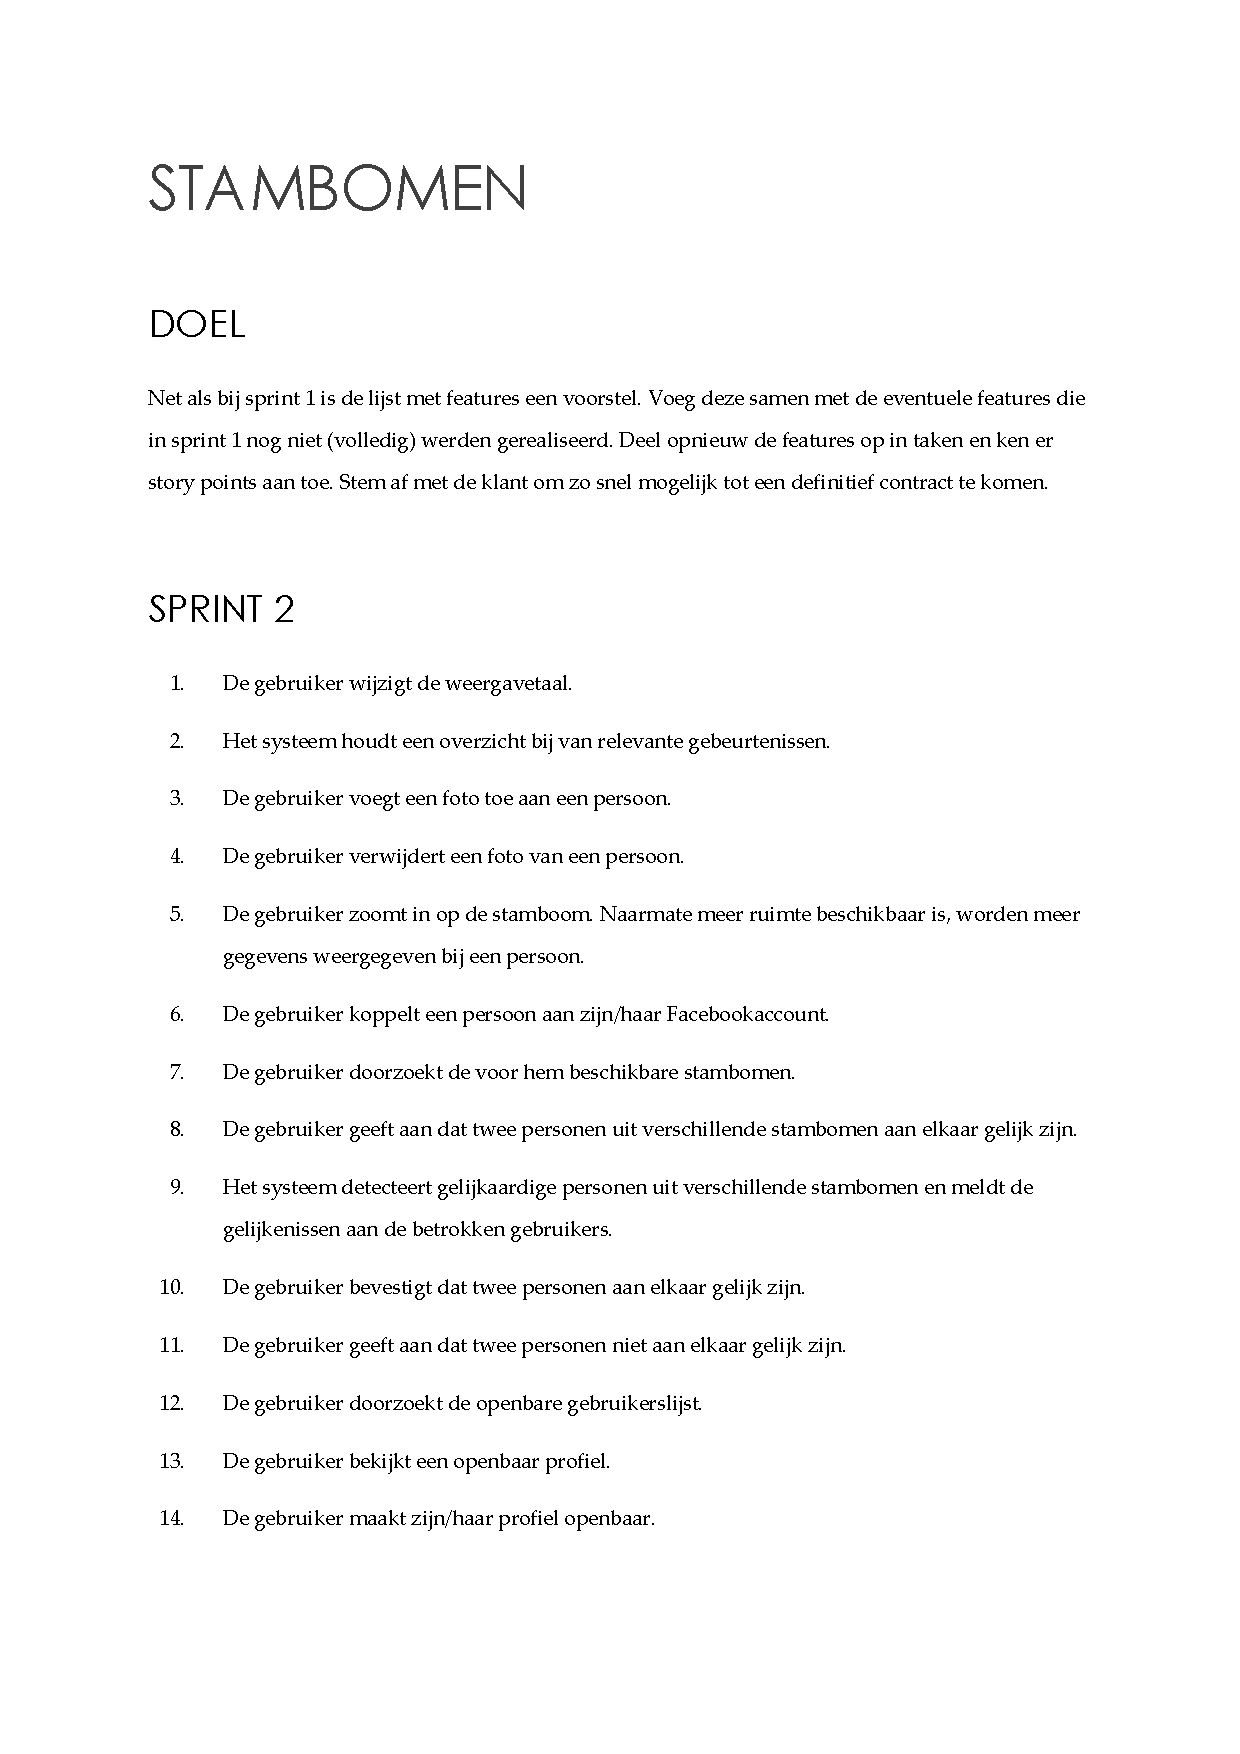
\includepdf[pages=-,pagecommand=\section{Opdracht sprint 2}, scale=0.80]{Files/stambomen-sprint2.pdf}

\end{document}

